\documentclass[10pt]{beamer}

% paquets pour le français
\usepackage[T1]{fontenc}
\usepackage[utf8]{inputenc}

% paquets autres
\usepackage{ulem}
\usepackage{listings}
\usepackage{xcolor}
\usepackage{hyperref}
\usepackage{graphicx}
\usepackage[figurename=Source]{caption}

% couleurs
\definecolor{light-grey}{RGB}{240,240,240}
\definecolor{dark-green}{RGB}{50, 80, 50}
\definecolor{cherry-red}{RGB}{200, 40, 40}

% theme général du diaporama
\usetheme{Madrid}
\usecolortheme[RGB={13, 87, 63}]{structure}

% configuration des zones de code
\lstset{
	backgroundcolor = \color{light-grey},  % Choose the background color
    commentstyle    = \color{dark-green},  % Highlighting comment
    keywordstyle    = \color{cherry-red},  % Highlighting keywords
    stringstyle     = \color{orange},      % Highlighting string
    inputencoding   = utf8,                % Input encoding
    extendedchars   = true,                % Extended ASCII
    breaklines      = true,                % Sets automatic line breaking
    language        = C,                   % Set language
    basicstyle      = \ttfamily\scriptsize,     % Set font size
    numbers         = left,                % Numeration
    numbersep       = 5pt,                 % Set numeration shift
    literate        =                      % Support additional characters
      {á}{{\'a}}1  {é}{{\'e}}1  {í}{{\'i}}1 {ó}{{\'o}}1  {ú}{{\'u}}1
      {Á}{{\'A}}1  {É}{{\'E}}1  {Í}{{\'I}}1 {Ó}{{\'O}}1  {Ú}{{\'U}}1
      {à}{{\`a}}1  {è}{{\`e}}1  {ì}{{\`i}}1 {ò}{{\`o}}1  {ù}{{\`u}}1
      {À}{{\`A}}1  {È}{{\'E}}1  {Ì}{{\`I}}1 {Ò}{{\`O}}1  {Ù}{{\`U}}1
      {ä}{{\"a}}1  {ë}{{\"e}}1  {ï}{{\"i}}1 {ö}{{\"o}}1  {ü}{{\"u}}1
      {Ä}{{\"A}}1  {Ë}{{\"E}}1  {Ï}{{\"I}}1 {Ö}{{\"O}}1  {Ü}{{\"U}}1
      {â}{{\^a}}1  {ê}{{\^e}}1  {î}{{\^i}}1 {ô}{{\^o}}1  {û}{{\^u}}1
      {Â}{{\^A}}1  {Ê}{{\^E}}1  {Î}{{\^I}}1 {Ô}{{\^O}}1  {Û}{{\^U}}1
      {œ}{{\oe}}1  {Œ}{{\OE}}1  {æ}{{\ae}}1 {Æ}{{\AE}}1  {ß}{{\ss}}1
      {ç}{{\c c}}1 {Ç}{{\c C}}1 {ø}{{\o}}1  {Ø}{{\O}}1   {å}{{\r a}}1
      {Å}{{\r A}}1 {ã}{{\~a}}1  {õ}{{\~o}}1 {Ã}{{\~A}}1  {Õ}{{\~O}}1
      {ñ}{{\~n}}1  {Ñ}{{\~N}}1  {¿}{{?`}}1  {¡}{{!`}}1
      {°}{{\textdegree}}1 {º}{{\textordmasculine}}1 {ª}{{\textordfeminine}}1
  }

% gestion des sections
\AtBeginSection[]{
	\begin{frame}
	\vfill
	\centering
	\begin{beamercolorbox}[sep=8pt, center]{title}
		\usebeamerfont{title}
  		\uline{\insertsectionhead}
  		\par
  	\end{beamercolorbox}
  	\vfill
  	\end{frame}
}

% gestion des blocs
\setbeamertemplate{blocks}[default]

% gestion des frames
\setbeamertemplate{frametitle continuation}{}
\setbeamersize{text margin left = 20px,text margin right = 20px} 

% informations
\author{\textit{Thomas CREUSET}}
\title{\uline{Pr\'esentation de TIPE}}
\subtitle{\textit{\'Etude et optimisation d’un outil d'ing\'enierie du b\^atiment}}
\date{\underline{\textit{num\'ero de candidat : 11909}}}

% document
\begin{document}

	% page de titre
	\frame{\titlepage}

	% sommaire
	\part{Sommaire}
	\begin{frame}
		\frametitle{\uline{Sommaire}}
		\tableofcontents
	\end{frame}

	% Choix du projet
	\section{Choix du projet}
	% frame 1.1
	\subsection{La construction en ville: un enjeu pour les ing\'enieurs}
	\begin{frame}
		\frametitle{\uline{Choix du projet :}}
		\framesubtitle{\textit{La construction en ville : un enjeu pour les ing\'enieurs}}
		\begin{columns}[t]
  			\begin{column}{5cm} 
				\begin{block}{}
					\uline{Objectifs de l'ing\'enieur :}
  					\begin{itemize}
						\item Stabilit\'e
						\item Durabilit\'e
						\item Accessibilit\'e
						\item Autres
					\end{itemize}
					\uline{Point d'int\'er\^et pour notre TIPE :}
					\begin{itemize}
						\item Stabilit\'e
					\end{itemize}
				\end{block}
  			\end{column}
 			\begin{column}{5cm}
 				\begin{figure}
   					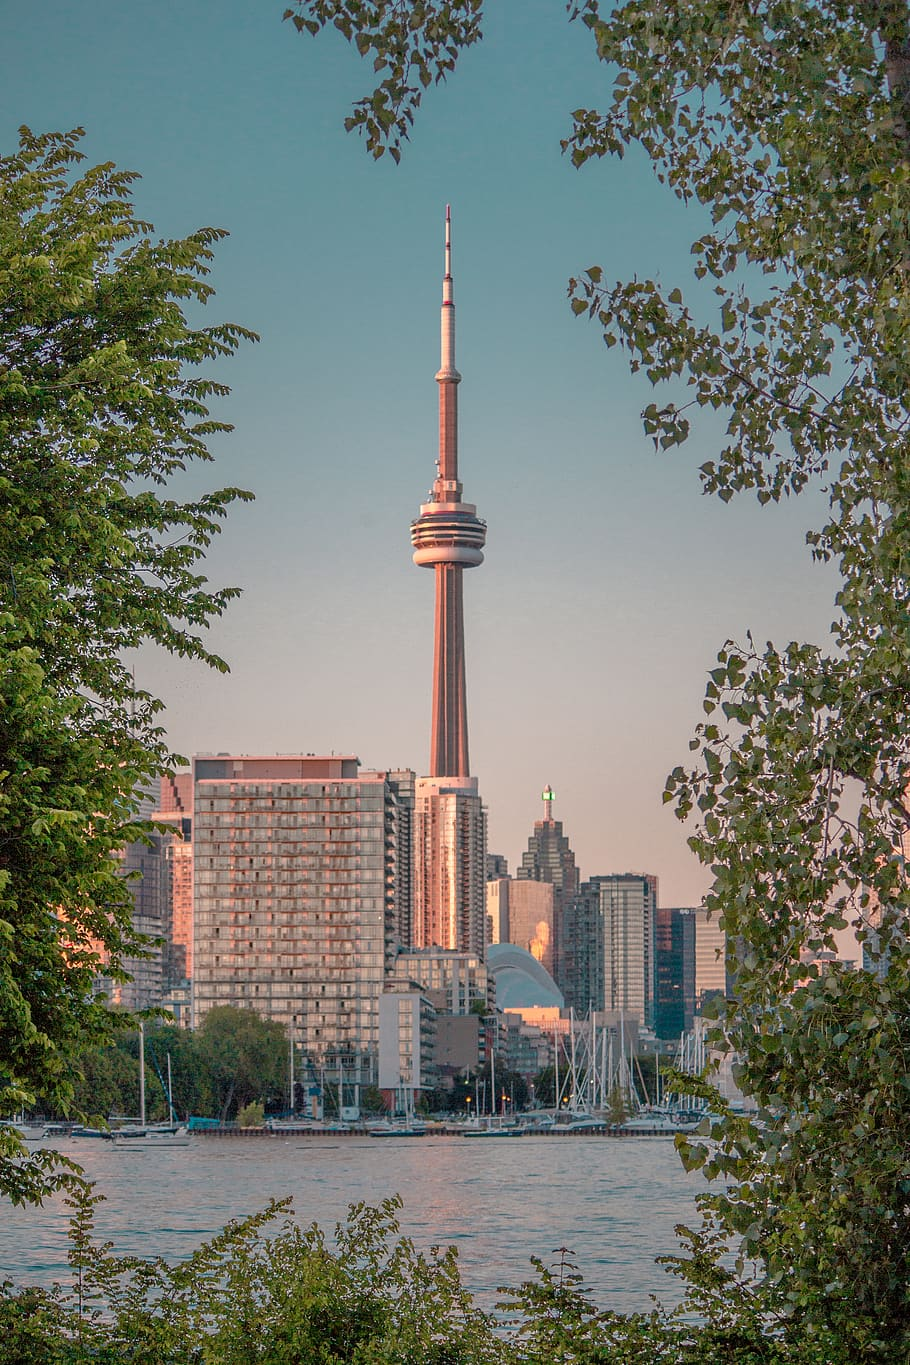
\includegraphics[scale = 0.125]{Images/city.png}
   					\caption{\href{https://www.wallpaperflare.com/city-portrait-buildings-skyscraper-tower-tall-toronto-wallpaper-eafsn}{wallpaperflare}}
				\end{figure}
			 \end{column}
 		\end{columns}
	\end{frame}
	%frame 1.2
	\subsection{Mod\'elisation informatique}
	\begin{frame}
		\frametitle{\uline{Choix du projet :}}
		\framesubtitle{\textit{Mod\'elisation informatique}}
		
		\begin{columns}[t]
  			\begin{column}{5cm} 
 				\begin{figure}
   					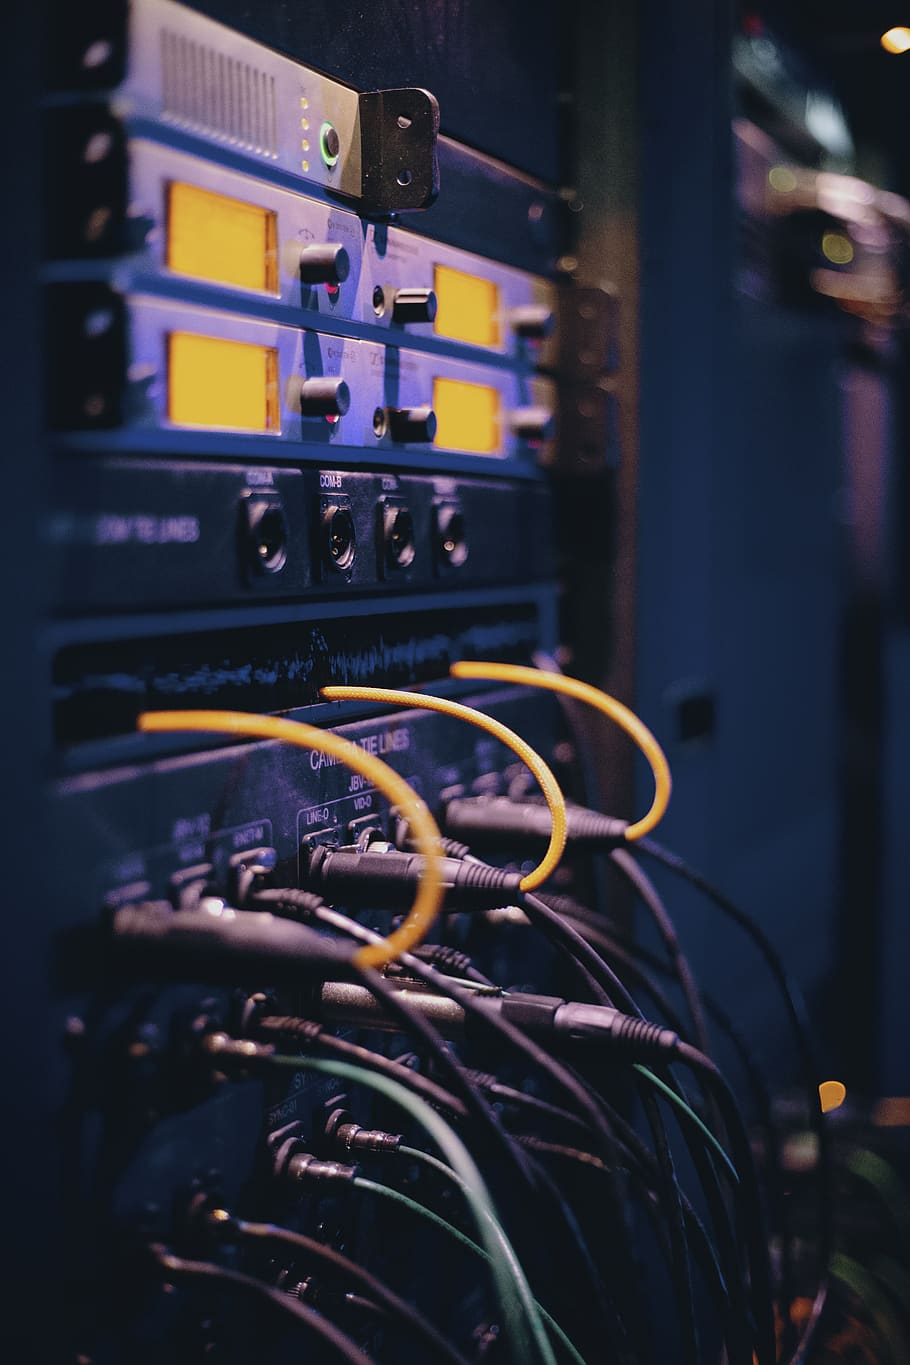
\includegraphics[scale = 0.125]{Images/cables.jpg}
   					\caption{\href{https://www.wallpaperflare.com/black-cables-connection-data-electronics-equipment-ethernet-wallpaper-aryet}{wallpaperflare}}
				\end{figure}
  			\end{column}
 			\begin{column}{5cm}
 				\begin{block}{}
 					\uline{Int\'er\^ets de la mod\'elisation informatique :}
					\begin{itemize}
						\item Co\^ut
						\item Dur\'ee
						\item Aspects sp\'ecifiques
						\item Param\'etrisation pr\'ecise
					\end{itemize}
				\end{block}
			 \end{column}
 		\end{columns}
	\end{frame}
	%frame 1.3
	\subsection{M\'ethode des \'el\'ements finis}
	\begin{frame}
		\frametitle{\uline{Choix du projet :}}-
		\framesubtitle{\textit{M\'ethode des \'el\'ements finis}}
		\centering
		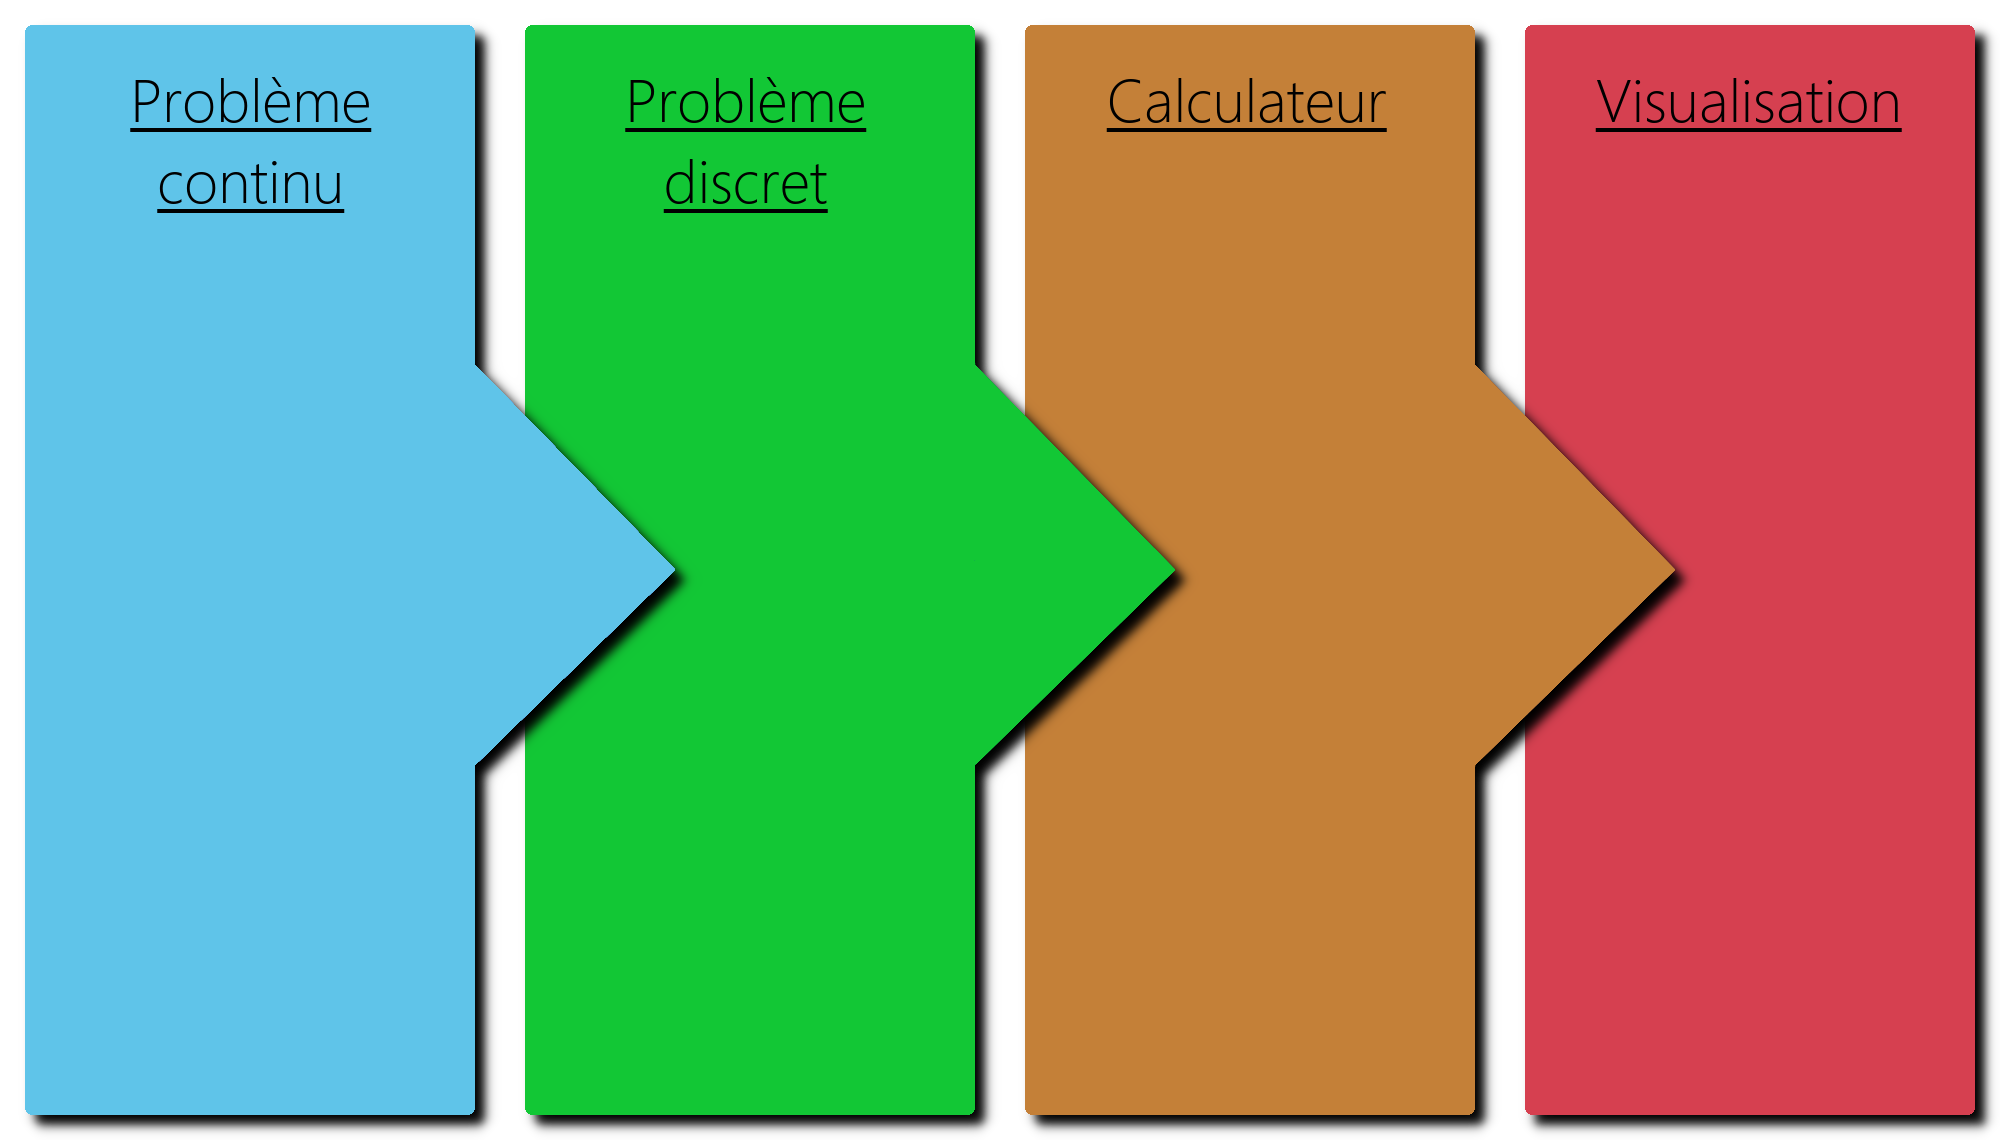
\includegraphics[scale=4.5]{Images/MethodeDesElementsFinis.png}
	\end{frame}

	% Méthode des éléments finis
	\section{M\'ethode des \'el\'ements finis}
	% frame 2.1
	\subsection{M\'ethode de Galerkine}
	\begin{frame}
		\frametitle{\uline{M\'ethode des \'el\'ements finis :}}
		\framesubtitle{\textit{M\'ethode de Galerkine}}
		\begin{columns}[t]
  			\begin{column}{5cm} 
				\begin{block}{}
  					\uline{Id\'ees sous-jacentes :}
   					\begin{itemize}
						\item Prendre un sous-ensemble V de l'ensemble des fonctions
						\item Calculer le projeté de notre solution sur V à l'aide de l'\'equation diff\'erentielle 
					\end{itemize}
					\uline{D\'efauts :}
					\begin{itemize}
						\item Connaissances math\'ematiques en calcul diff\'erentiel pouss\'e
						\item Difficile \`a g\'en\'eraliser
					\end{itemize}
				\end{block}
  			\end{column}
 			\begin{column}{5cm}
 				\begin{figure}
   					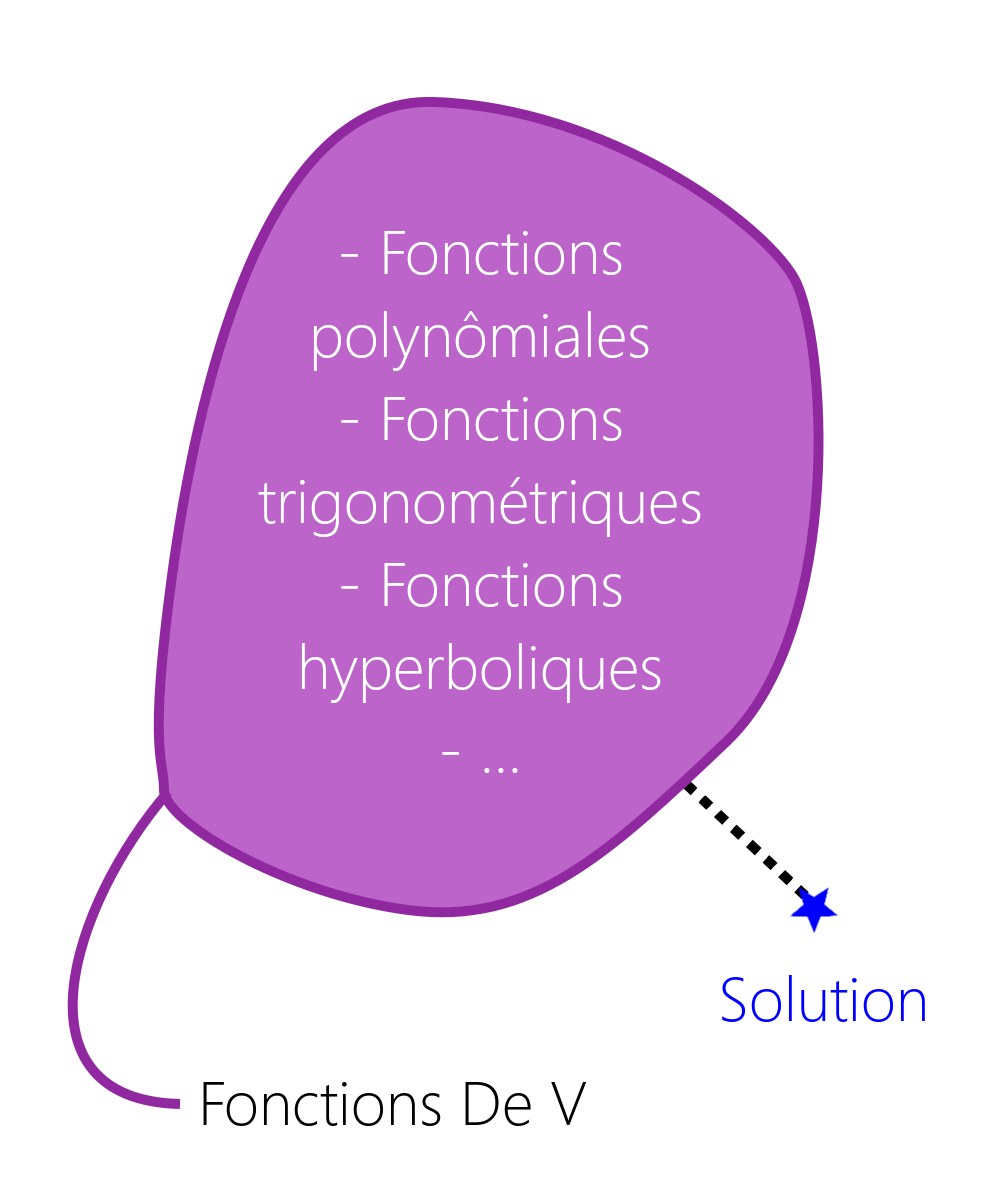
\includegraphics[scale = 0.58]{Images/Galerkine.png}
				\end{figure}
			 \end{column}
 		\end{columns}
	\end{frame}
	% frame 2.2
	\subsection{M\'ethode des ressorts}
	\begin{frame}
		\frametitle{\uline{M\'ethode des \'el\'ements finis :}}
		\framesubtitle{\textit{M\'ethode des ressorts}}
		\centering
  		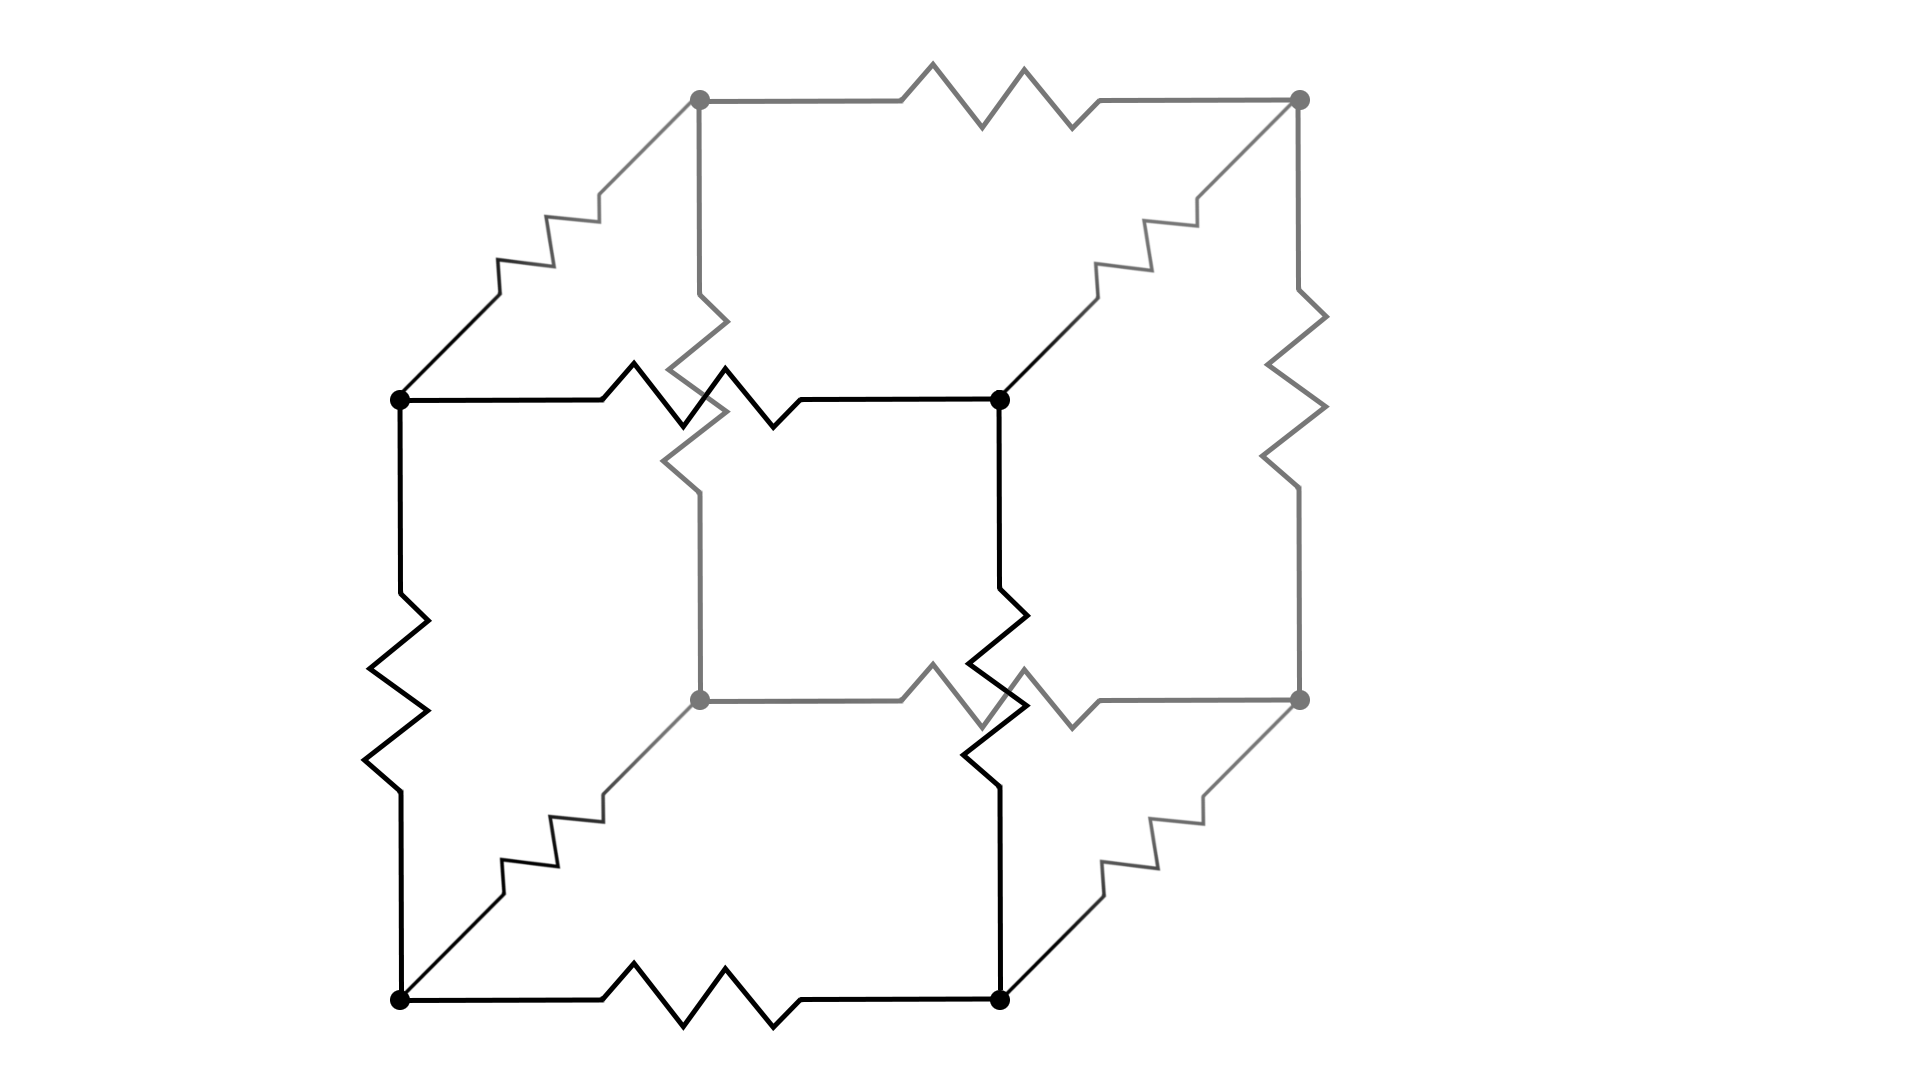
\includegraphics[scale=0.84]{Images/cube.png}
	\end{frame}
	% frame 2.3
	\subsection{Loi de Hooke}
	\begin{frame}
		\frametitle{\uline{M\'ethode des \'el\'ements finis :}}
		\framesubtitle{\textit{Loi de Hooke}}
		\begin{block}{Loi de Hooke}
			\begin{equation}
  				\vec{\mathcal{F}} = - k \cdot \Delta \ell \cdot \vec{u}
  			\end{equation}
		\end{block}
		\begin{block}{Constante de raideur}
			\begin{equation}
				k = \frac{\mathrm{A} \cdot \mathrm{E}}{\mathrm{L}}
			\end{equation}
			avec :\\
  			\begin{itemize}
  				\item $\mathrm{A}$ : l'aire de la section de la poutre
  				\item $\mathrm{E}$ : le module de Young du matériel
  				\item $\mathrm{L}$ : la longueur de la poutre
  			\end{itemize}
		\end{block}
	\end{frame}
	%frame 2.4
	\subsection{G\'en\'eralisation, matrice de raideur}
	\begin{frame}
		\frametitle{\uline{M\'ethode des \'el\'ements finis :}}
		\framesubtitle{\textit{G\'en\'eralisation, matrice de raideur}}
		\begin{block}{Loi de Hooke matricielle}
			\begin{equation}
  				F = K \cdot U
  			\end{equation}
		\end{block}
		\begin{block}{Forme d\'etaill\'ee}
			\begin{equation}
				\begin{pmatrix}
				F_c \\
				F_i
				\end{pmatrix}
				=
				\begin{pmatrix}
				K_1 & K_2 \\
				K_3 & K_4
				\end{pmatrix}
				\cdot
				\begin{pmatrix}
				U_i \\
				U_c
				\end{pmatrix}
			\end{equation}
			Conditions aux limites pour la solution d'une \'equation diff\'erentielle :
			\begin{itemize}
				\item Neumann : information sur ses dérivées (forces connues)
				\item Dirichlet : information sur sa valeur (déplacments connus)
			\end{itemize}
		\end{block}
	\end{frame}
	%frame 2.5
	\subsection{Deux astuces}
	\begin{frame}
		\frametitle{\uline{M\'ethode des \'el\'ements finis :}}
		\framesubtitle{\textit{Deux astuces}}
		\begin{block}{R\'ecup\'eration des forces et des d\'eplacements inconnus}
			\begin{align}
				&F_c = K_1 \cdot U_i + K_2 \cdot U_c\\
				&\textit{d'o\`u : } U_i = K_1^{-1} \cdot (F_c - K_2 \cdot U_c)\\
				&\textit{et : } F_i = K_3 \cdot U_i + K_3 \cdot U_c
			\end{align}
		\end{block}
		\begin{block}{Rotation vers cas par d\'efault}
			\begin{columns}[t]
  				\begin{column}{5cm}
  					\centering
  					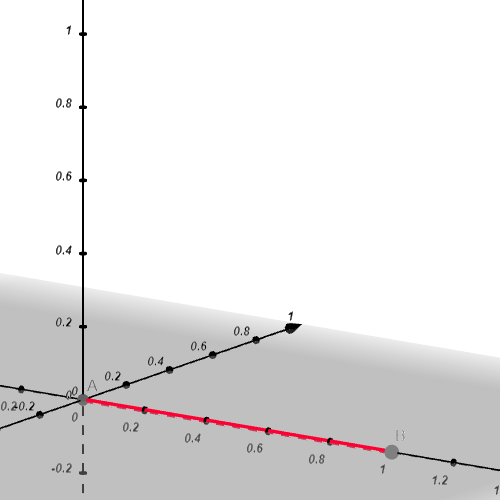
\includegraphics[scale=0.2]{Images/CasDeBase.png}
  				\end{column}
 				\begin{column}{5cm}
 				 	\centering
 				 	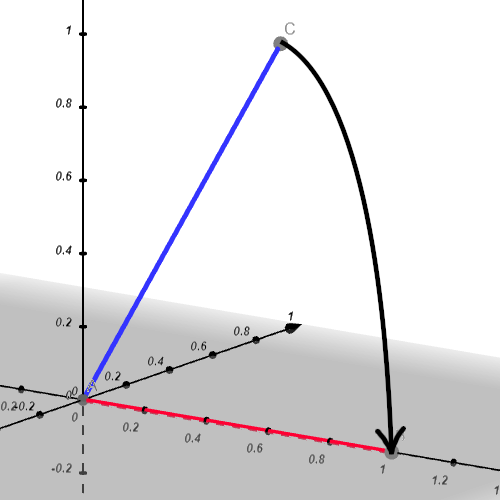
\includegraphics[scale=0.2]{Images/CasFinal.png}
				 \end{column}
 			\end{columns}
		\end{block}
	\end{frame}
	%frame 2.6
	\subsection{Affichage}
	\begin{frame}
		\frametitle{\uline{M\'ethode des \'el\'ements finis :}}
		\framesubtitle{\textit{Affichage}}
		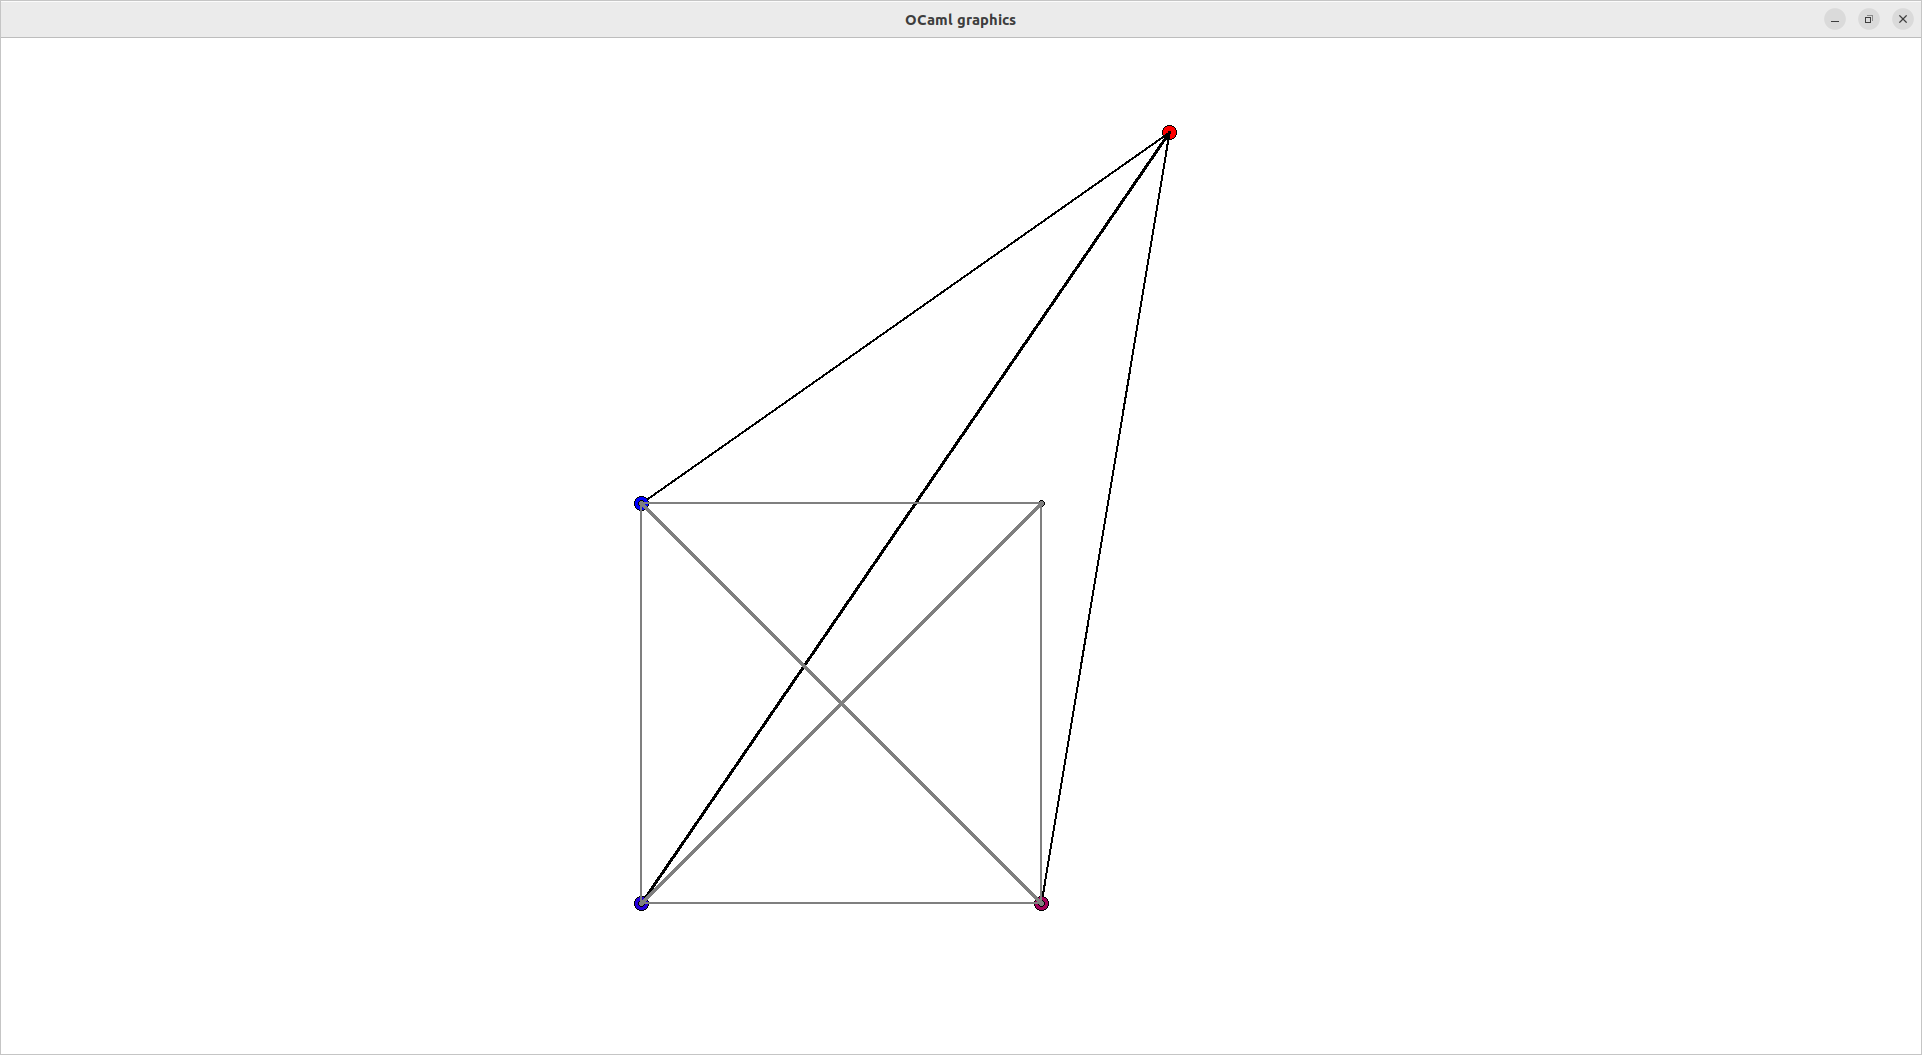
\includegraphics[scale = 0.17]{Images/Copium.png}
	\end{frame} 

	% Optimisation
	\section{Optimisation}
	% frame 3.1
	\subsection{Analogique et num\'erique, d\'efaults et qualit\'es}
	\begin{frame}
		\frametitle{\uline{Optimisation :}}
		\framesubtitle{\textit{Analogique et num\'erique, d\'efaults et qualit\'es}}
		\uline{Points de divergence des m\'ethode :}
		\begin{itemize}
     		\item Vitesse
     		\item Co\^ut
     		\item Pr\'ecision des calculs
     		\item Flexibilit\'e du param\`etrage
 		\end{itemize}
	\end{frame}
	%frame 3.2
	\subsection{Retours exp\'erimentaux}
	\begin{frame}
		\frametitle{\uline{Optimisation :}}
		\framesubtitle{\textit{Retours exp\'erimentaux}}
		Pas encore fait
	\end{frame}
	%frame 3.3
	\subsection{Une solution inattendue et conclusion}
	\begin{frame}
		\frametitle{\uline{Optimisation :}}
		\framesubtitle{\textit{Une solution inattendue}}
		\centering
  		\uline{\textbf{La m\'ecanique quantique une solution pour le futur}}
  		\par
  		\vfill
		Algorithme d'inversion HHL (H.arrow H.assidim L.loyd) :
		\begin{quote}
			<<HHL apporte une amélioration significative, de O(n) à O(log(n)).>>\footnote{\textit{L’apport des technologies quantiques en intelligence artificielle : vers une acculturation et une compr\'ehension des enjeux du quantique pour l’arm\'ee de l’air et de l’espace}, Commandant Campo Marie-\'Elisabeth, Bureau num\'erique de l’arm\'ee de l’air et de l’espace}
		\end{quote}
	\end{frame}
	
	% Annexes
	\section{Annexes}
	% partie C
	\subsection{Code C}
	\begin{frame} [allowframebreaks]
		\frametitle{\uline{Annexes :}}
		\framesubtitle{\textit{Code C : standard\_lib.h}}
		\lstinputlisting{Code/C/standard_lib.h}
	\end{frame}
	\begin{frame}[allowframebreaks]
		\frametitle{\uline{Annexes :}}
		\framesubtitle{\textit{Code C : module\_matrice.h}}
		\lstinputlisting{Code/C/module\_matrice.h}
	\end{frame}
	\begin{frame}[allowframebreaks]
		\frametitle{\uline{Annexes :}}
		\framesubtitle{\textit{Code C : module\_matrice.c}}
		\lstinputlisting{Code/C/module\_matrice.c}
	\end{frame}
	\begin{frame}[allowframebreaks]
		\frametitle{\uline{Annexes :}}
		\framesubtitle{\textit{Code C : main.c}}
		\lstinputlisting{Code/C/main.c}
	\end{frame}
	% partie C
	\subsection{Code Ocaml}
	\begin{frame} [allowframebreaks]
		\frametitle{\uline{Annexes :}}
		\framesubtitle{\textit{Code Ocaml : Affichage\_FEM\_3D.ml}}
		\lstinputlisting[language = caml]{Code/Ocaml/Affichage_FEM_3D.ml}
	\end{frame}
\end{document}

